\documentclass[aspectratio=169,10pt]{beamer}
\usetheme{default}
\usecolortheme{seahorse}
\setbeamertemplate{navigation symbols}{}
\setbeamertemplate{footline}[frame number]
\usepackage[T1]{fontenc}
\usepackage{booktabs,graphicx}
\graphicspath{{../../}}
\title{Design Pattern Analysis in a Next.js-Based Video Streaming Application}
\subtitle{23CSE455 Design Patterns --- Case Study, Team A12}
\author{Swaminathan A \and Anna Ouseph \and Leya Paul \and Pooja Sathyan \and Rahul Rajan}
\date{October 2026}
\begin{document}

\begin{frame}\titlepage\end{frame}

\begin{frame}{Application under study}
\begin{columns}[T]
\column{0.40\textwidth}
\small
\begin{itemize}
\item \textbf{netflx-web} (sadmann7), Netflix clone
\item Next.js 13.4 app router, tRPC 10, NextAuth 4, Prisma 4 (MySQL), Stripe, Zustand, React Query, TMDB API
\item Baseline commit \texttt{676e5dd} (2024-06-12)
\item No LICENSE file --- academic analysis only
\item Seven areas: user management, catalogue, subscription, recommendation, authentication, content access, caching
\end{itemize}
\column{0.58\textwidth}
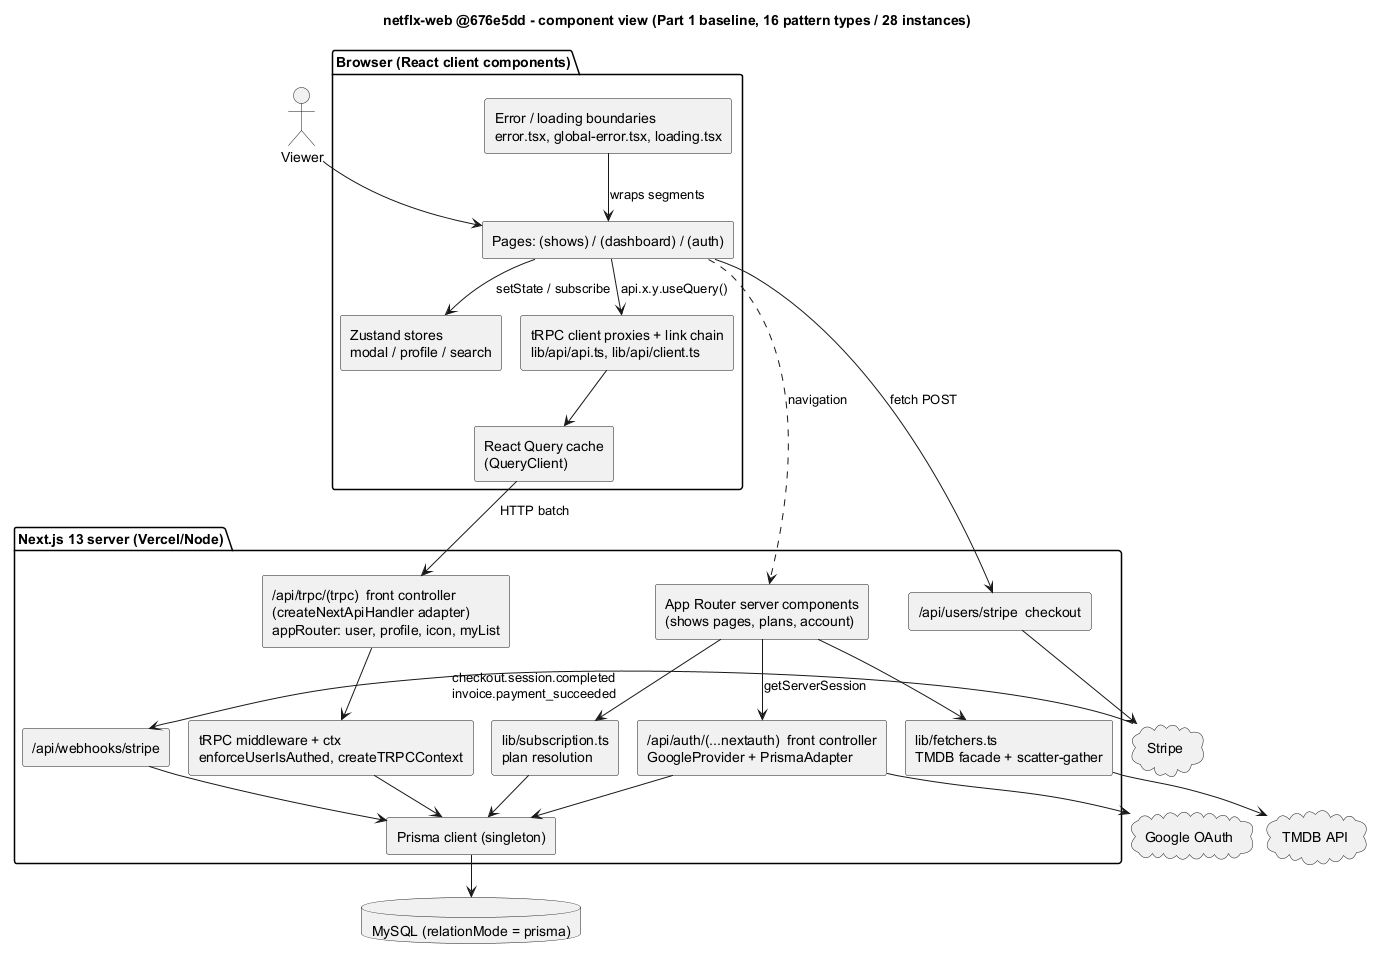
\includegraphics[width=\linewidth]{Part1/pattern_architecture/00_architecture.png}
\end{columns}
\end{frame}

\begin{frame}{Part 1 --- pattern catalogue at the baseline (two passes)}
\scriptsize
\begin{tabular}{@{}lp{8.4cm}cc@{}}\toprule
Pattern & Instances & \# & Concr.\\\midrule
Chain of Responsibility & Authenticated Procedure Pipeline; \textbf{tRPC Client Link Chain} & 2 & 3\\
Singleton & Shared Prisma Client; Stripe API Client & 2 & 2\\
Observer & Show Modal Selection; Active Profile Selection; Search Results; \textbf{Search Input DOM Listeners} & 4 & 17\\
Decorator & Persisted Profile Store (devtools(persist(\dots))) & 1 & 3\\
Adapter & NextAuth Prisma Persistence Adapter; \textbf{tRPC Next.js API Handler Adapter} & 2 & 2\\
Strategy & Sign-in Provider Strategy; \textbf{Wire Serialization Transformer} & 2 & 2\\
Facade / Composite & TMDB Catalogue Facade / API Router Tree & 1+1 & 1+5\\
Proxy & 2 tRPC client proxies; Environment Secret Guard & 3 & 3\\
Read-Through Cache & My List Query Cache; \textbf{Profile and Account Query Cache} & 2 & 2\\
\textbf{Front Controller} & tRPC API Front Controller; NextAuth Auth Route Front Controller & 2 & 2\\
\textbf{Builder / Context Object} & tRPC Procedure Builder / tRPC Request Context & 1+1 & 2+1\\
\textbf{Error / Suspense Boundary} & Shows Segment + Root Global Error Boundary / Shows Loading Placeholder & 2+1 & 2+1\\
\textbf{Scatter-Gather} & TMDB Row Scatter-Gather & 1 & 2\\\midrule
\textbf{16 types} & first pass 10 types / 15 instances; second pass (bold) +6 / +13 & \textbf{28} & \textbf{50}\\\bottomrule
\end{tabular}
\par\smallskip 11 rejected (e.g.\ dead caching proxy, Suspense around non-suspending forms), 5 uncertain (e.g.\ Stripe webhook). 156 cited ranges checked by script: 0 problems.
\end{frame}

\begin{frame}{Second pass --- what the area-driven first pass missed}
\begin{columns}[T]
\column{0.5\textwidth}\small
\begin{itemize}
\item Read \emph{every} in-scope file, not only area entry files
\item Verified dependency roles in the exact versions (\texttt{npm pack} @trpc/* 10.28.0, next-auth 4.22.1, next 13.4.4)
\item Found the infrastructure patterns: two \textbf{front controllers}, an immutable \textbf{builder}, a \textbf{context object}, error and \textbf{Suspense boundaries}, \textbf{scatter-gather}
\item Corrected one existing record: the pages-router client's own link chain is never executed
\end{itemize}
\column{0.48\textwidth}
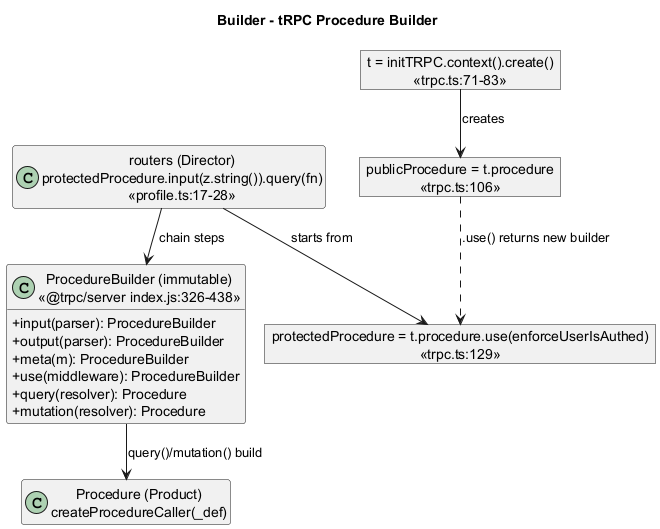
\includegraphics[width=\linewidth]{Part1/pattern_architecture/20_builder_trpc_procedure_builder.png}
\end{columns}
\end{frame}

\begin{frame}{Example: Environment Secret Guard (protection proxy)}
\begin{columns}[T]
\column{0.5\textwidth}\small
\begin{itemize}
\item \texttt{env = new Proxy(parsed.data, \{get\})} in \texttt{env.mjs:92-105}
\item On the client, any non-\texttt{NEXT\_PUBLIC\_} read throws
\item Explains a smell found in Part 2: plan data was duplicated because the server list reads secrets
\end{itemize}
\column{0.48\textwidth}
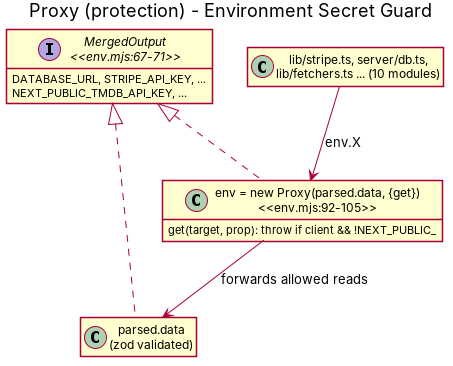
\includegraphics[width=\linewidth]{Part1/pattern_architecture/15_proxy_environment_secret_guard.png}
\end{columns}
\end{frame}

\begin{frame}{Part 2 --- three changes}
\small
\begin{tabular}{@{}p{3.3cm}p{6.6cm}p{3.6cm}@{}}\toprule
Change & What & Tests\\\midrule
CH01 premium + Ultra plan & tier-based premium titles, Ultra (7 profiles), subscription middleware & 29/29\\
CH02 regional restrictions & licences per country, geo header, server-side row filtering & 45/45\\
CH03 parental control & KIDS / TEEN / ADULT rating per profile & 65/65\\\bottomrule
\end{tabular}
\par\medskip
\begin{itemize}
\item Characterization tests written first and run on the \emph{original} code (19/19)
\item New student-added \textbf{Content Access Rule Chain}: Region $\rightarrow$ Maturity $\rightarrow$ Premium (hide before lock)
\item Existing tRPC middleware chain extended with \texttt{attachSubscription}; immutable builders kept \texttt{protectedProcedure} unchanged
\end{itemize}
\end{frame}

\begin{frame}{Pattern evolution}
\begin{columns}[T]
\column{0.5\textwidth}\small
\begin{tabular}{@{}lcccc@{}}\toprule
Snapshot & Types & Inst. & Concr.\\\midrule
baseline & 16 & 28 & 50\\
CH01 & 17 & 30 & 56\\
CH02 & 17 & 30 & 57\\
CH03 & 17 & 30 & 60\\\bottomrule
\end{tabular}
\par\medskip
\begin{itemize}
\item New: Content Access Rule Chain (CoR), Access Rule Evaluation Template (Template Method)
\item Extended: auth pipeline, router tree, profile observers, tRPC front controller, procedure builder, request context
\item Modified: TMDB facade, TMDB scatter-gather, search observer; none removed
\end{itemize}
\column{0.48\textwidth}
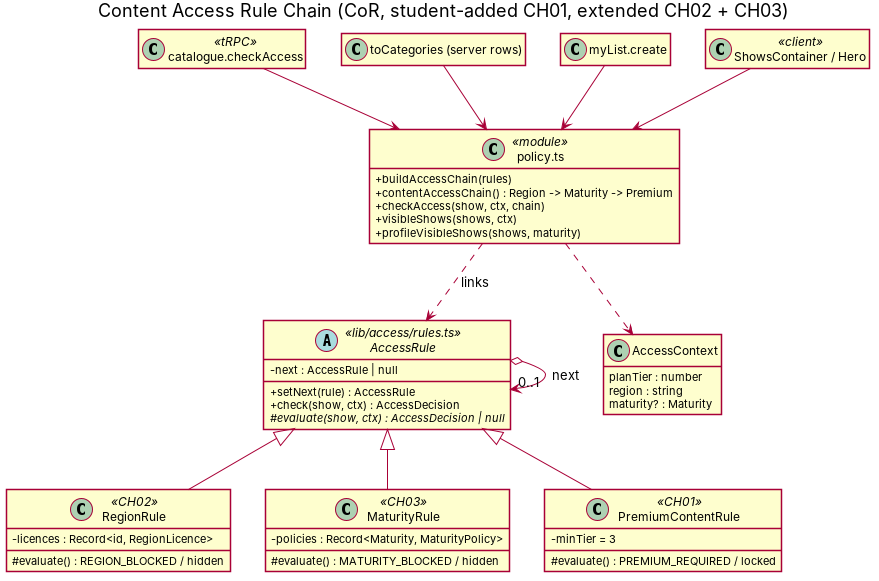
\includegraphics[width=\linewidth]{Part2/diagrams/01_content_access_rule_chain_CH03.png}
\end{columns}
\end{frame}

\begin{frame}{Refactoring --- real smells, measured with the same tool}
\small
\begin{tabular}{@{}p{5.2cm}p{4.2cm}rr@{}}\toprule
Smell & Technique & Before & After\\\midrule
Duplicated plan data (UI vs server, already drifted) & shared client-safe catalogue & 139 NLOC & 123 (+1 plan)\\
Copy-pasted TMDB fetch blocks (two scatter-gathers) & rows as data + \texttt{fetchRows} & max CCN 9 & 3\\
Same row array in 3 pages & \texttt{GENRE\_ROWS} + \texttt{toCategories} & 174 NLOC & 116\\
Duplicated zod schema / lookups in My List & Extract Variable / Function & 169 NLOC & 114\\\bottomrule
\end{tabular}
\par\medskip
Whole \texttt{src/}: 6694 $\rightarrow$ 6916 NLOC (+3.3\%), avg CCN 2.31 $\rightarrow$ 2.26. LOC alone does not prove better design; the evidence is behaviour preserved by tests.
\end{frame}

\begin{frame}{Part 3 --- four languages, one shared fixture, 16 pattern types}
\small
\begin{tabular}{@{}lrrrr@{}}\toprule
 & Java & Python & JavaScript & C++\\\midrule
cases passed (16 problems) & 177/177 & 177/177 & 177/177 & 177/177\\
total source LOC & 899 & 568 & 623 & 1019\\
max function CC & 11 & 9 & 10 & 11\\
median of median process times (ms) & 116.8 & 50.1 & 59.2 & 16.2\\\bottomrule
\end{tabular}
\par\medskip
\begin{itemize}
\item Proxy: JS \texttt{Proxy} trap $\approx$ source; Python \texttt{\_\_getattr\_\_}; Java \texttt{reflect.Proxy}; C++ plain class
\item Builder: immutability by spread/\texttt{freeze} (JS), tuples (Py), \texttt{List.copyOf}/records (Java), value copies + const methods (C++)
\item Scatter-Gather: \texttt{Promise.all} \emph{is} the pattern in JS (10 NLOC); C++ starts real threads (\texttt{std::async})
\item Times (Windows 11) are start-up dominated: they compare runtimes, not patterns
\end{itemize}
\end{frame}

\begin{frame}{LLM use and verification}
\small
\begin{itemize}
\item Session 1 (claude.ai, Claude Opus 5.5, 2026-10-10): Parts 1--3. Session 2 (Claude Code, Claude Opus 5.5, 2026-10-29/30): exhaustive second pass, 6 new Part 3 problems, full re-run
\item Prompts: \texttt{Part1/Part1\_prompt.txt}, \texttt{Part2/Part2\_prompt.text}, \texttt{Part3/llm/part3\_prompt.txt}; records in each part's \texttt{llm.csv}
\item Errors found by checking: missed instances (env proxy; 13 infrastructure instances), wrong line ranges, a wrong transport role, an inactive link chain claimed active, three first code drafts that did not compile or follow React's reset rule
\item All generated code is covered by tests (65 app tests, 708 cross-language checks)
\end{itemize}
\end{frame}

\begin{frame}{Findings}
\small
\begin{itemize}
\item 16 pattern types / 28 instances at the baseline; most are inherited from frameworks (tRPC, zustand, NextAuth, React Query, Next.js) and configured, not written
\item An area-driven first pass misses the infrastructure layer --- read every file
\item Recommendation has no pattern because it has no logic
\item A chain of rules absorbed premium, region and parental control with one class each
\item Pre-existing issues: client-side PIN check, missing ownership checks on profile / My List, dead caching proxy, two parallel tRPC clients
\item Limits: no end-to-end run with real Stripe / TMDB / Google; sample licence data
\end{itemize}
\end{frame}

\end{document}
